\section{De AX5140 Drive}

In figuur \ref{fig:AX5140} is een afbeelding van de motordrive die momenteel in de testkast zit. Deze drive heeft hiernaast nog een \gls{AX5801}-0200 veiligheidskaart geïnstalleerd wat de drive ertoe in staat brengt om ook bepaalde veiligheidsfuncties te configureren zoals de \gls{STO} (Safe Torque Off) functie en de \gls{SS1} stop functie om veilig en snel tot stilstand te komen in geval van nood. \cite{web:AX5801}

\vspace{0.5cm}

Daarnaast ondersteunt de \gls{AX5140} standaard niet alle encoder types hiervoor is een extra option card geïnstalleerd in de drive dit is de \gls{AX5701} encoder option card waardoor encoders zoals EnDat en Hiperface wel aangesloten kunnen worden. De \gls{AX5702} die te zien is in figuur 1 is in principe hetzelfde als de \gls{AX5701} alleen heeft de \gls{AX5702} een extra port die de \gls{AX5701} niet heeft. 

\vspace{0.5cm}

Alle spindels die Voortman wil gaan testen kunnen wel aangesloten worden en deze kunnen ook worden gemonteerd op de testkast. Maar momenteel is er maar één parameter set voor één type spindel op het programma van de testkast. Het is nog niet mogelijk om geautomatiseerd andere parametersets in te laden in de motordrive.

\vspace{0.5cm}

Op het moment wanneer er nieuwe parameters in de drive geladen moeten worden zal dit handmatig moeten gebeuren middels een driverproject in TwinCAT XAE of Visual studio met een TwinCAT extensie.


\begin{figure}[h]
	\centering
	\begin{minipage}{0.32\textwidth}
		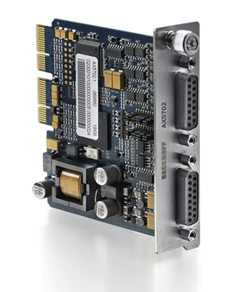
\includegraphics[width=\linewidth]{AX5702}
		\vspace{0pt}
		\caption{AX5702 Encoder option card \cite{web:AX5701}}
		\label{fig:AX5702}
	\end{minipage}
	\hfill
	\begin{minipage}{0.32\textwidth}
		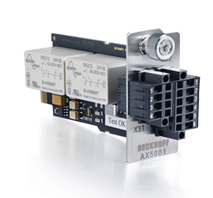
\includegraphics[width=\linewidth]{AX5801}
		\vspace{0pt}
		\caption{AX5801-0200 Safety card \cite{web:AX5801}}
		\label{fig:AX5801}
	\end{minipage}
	\hfill
	\begin{minipage}{0.32\textwidth}
		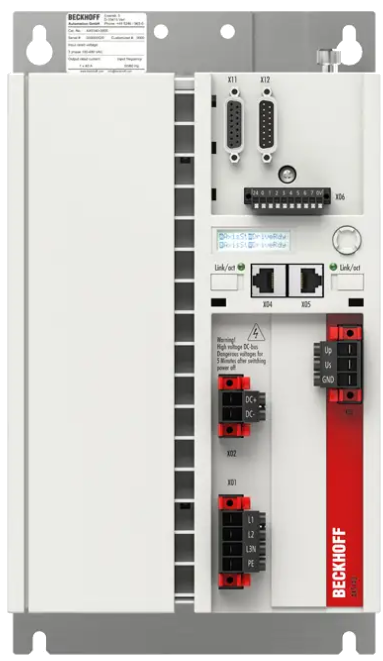
\includegraphics[width=\linewidth]{AX5140}
		\vspace{0pt}
		\caption{Beckhoff AX5140 drive \cite{web:AX5140Drive}}
		\label{fig:AX5140}
	\end{minipage}
\end{figure}

\newpage

\subsection{Motor vergelijking}

Om te kunnen weten of de huidige drive de motoren aan kan op basis van het vermogen van de motoren moeten de specificaties van de motoren worden vergeleken met de specificaties van de drive. De volgende motoren wil Voortman gaan testen op de testkast:

\begin{table}[H]
	\caption{Driver maximum ampère en voltage}
	\label{tab:AX5140Max}
	\centering
	\begin{tabular}{|c|c|}
		\hline
		\textbf{AX5140} & \textbf{Value} \\
		\hline
		\textbf{Rated Current} & 40 \gls{A} \\
		\textbf{Peak Current} & 80 \gls{A} \\
		\textbf{Voltage} & 400\gls{V} \\
		\hline
	\end{tabular}
\end{table}

\begin{table}[H]
	\caption{MAD100D Motor specificaties}
	\label{tab:MAD100D}
	\centering
	\begin{tabular}{|c|c|}
		\hline
		\textbf{MAD100D-0250-SA-C0-AK0-35-N3} & \textbf{Value} \\
		\hline
		\textbf{Rated Current} & 32.4 \gls{A} \\
		\textbf{Peak Current} & 64 \gls{A} \\
		\textbf{Voltage} & 400\gls{V} \\
		\hline
	\end{tabular}
\end{table}

\begin{table}[H]
	\caption{MAD130C Motor specificaties}
	\label{tab:MAD130C}
	\centering
	\begin{tabular}{|c|c|}
		\hline
		\textbf{MAD130C-0150-SA-S2-AP0-05-N1} & \textbf{Value} \\
		\hline
		\textbf{Rated Current} & 31.8 \gls{A} \\
		\textbf{Peak Current} & 93.3 \gls{A} \\
		\textbf{Voltage} & 400\gls{V} \\
		\hline
	\end{tabular}
\end{table}

\begin{table}[H]
	\caption{HQL100X Motor specificaties}
	\label{tab:HQL100X}
	\centering
	\begin{tabular}{|c|c|}
		\hline
		\textbf{HQL100X} & \textbf{Value} \\
		\hline
		\textbf{Rated Current} & 10.16 \gls{A} \\
		\textbf{Peak Current} & 19.7 \gls{A} \\
		\textbf{Voltage} & 400\gls{V} \\
		\hline
	\end{tabular}
\end{table}

\begin{table}[H]
	\caption{MSK101D Motor specificaties}
	\label{tab:HQL100X}
	\centering
	\begin{tabular}{|c|c|}
		\hline
		\textbf{MSK101D-0450-NN-M1-AP0-NNNN} & \textbf{Value} \\
		\hline
		\textbf{Rated Current} & 41.7 \gls{A} \\
		\textbf{Peak Current} & 187.7 \gls{A} \\
		\textbf{Voltage} & 400\gls{V} \\
		\hline
	\end{tabular}
\end{table}

\begin{table}[H]
	\caption{MS2N10 Motor specificaties}
	\label{tab:HQL100X}
	\centering
	\begin{tabular}{|c|c|}
		\hline
		\textbf{MS2N10-D0BNN-AMVK0-NNNNN-NN} & \textbf{Value} \\
		\hline
		\textbf{Rated Current} & 28.2 \gls{A} \\
		\textbf{Peak Current} & 102.5 \gls{A} \\
		\textbf{Voltage} & 400\gls{V} \\
		\hline
	\end{tabular}
\end{table}


Naast deze spindels maakt Voortman ook nog gebruik van spindels van WEISS deze zijn echter te lang en passen niet op de huidige testkast. Voortman wil deze ook niet gaan reviseren daarom worden deze spindels tijdens het gehele onderzoek buiten beschouwing gelaten.

\vspace{0.5cm}

Zoals te zien in de tabellen zijn er een aantal motoren die de motordrive niet aan kan op maximaal vermogen. Echter zal er geen mechanische belasting zijn waardoor deze motoren waarschijnlijk zonder problemen zullen presteren. Maar dit zal moeten blijken bij het testen van de motor. Wanneer dit niet het geval is zal er een sterkere drive moeten komen of er kan niet het maximale uit de motor gehaald kunnen worden tijdens de test of de motor zal compleet uitgesloten moeten worden van de testkast.
